%نام و نام خانوادگی:
%شماره دانشجویی: 
\مسئله{}



\پاسخ{
ابتدای هر 
\lr{object layout}
vtable آن قرار دارد که یک نشانگر به آن است.
سپس در بایت‌های بعدی فیلدهای مربوط به کلاس‌های پدر به ترتیب می‌آید.(فیلدهایی که تا الان نیامدند)و در انتها 
هم فیلدهای مختص به کلاس مربوطه می‌آید که در بقیه فیلد‌ها نباشد.
در vtable کلاس مربوطه ابتدا اطلاعات کلاس می‌آید و سپس برای هر تبع یک pointer به کد آن را نگه میداریم.
و در ادامه برای هر کلاس پدر یک pointer به کلاس پدر آن نگه می‌داریم.
\newline
هنگام استفاده از یک آبجکت از کلاس همان آبجکت مشکلی وجود ندارد. برای دسترسی به فیلد‌ها مانند وراثت یگانه عمل می‌کنیم و هنگام فراخوانی توابع آن کلاس اگر
 تابع مورد نظر در آن کلاس بود که فراخوانی می‌شود اگر نبود در vtable پدران کلاس جستجو می‌کنیم. اگر بود که کال می‌شود و اگر در هیچ کلاس پدری وجود نداشت خطای مورد نظر ارسال ایجاد می‌شود.
 \newline
 
\begin{enumerate}
	\item
		\begin{figure}[H]
			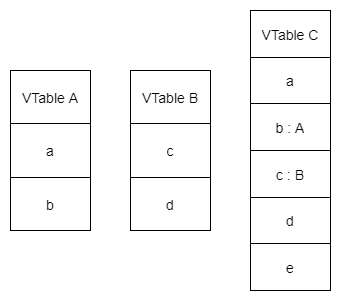
\includegraphics[scale=0.5]{commons/21.png}
		\end{figure}
	\item
		\begin{figure}[H]
			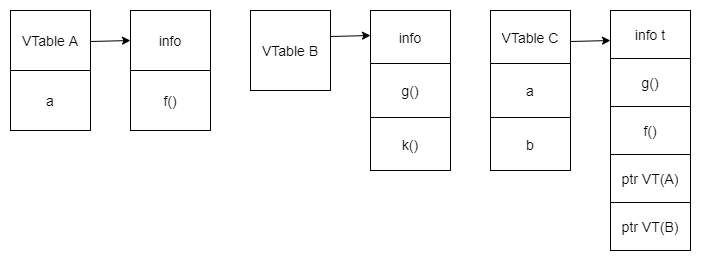
\includegraphics[scale=0.5]{commons/22.png}
		\end{figure}
	\item
		\begin{figure}[H]
			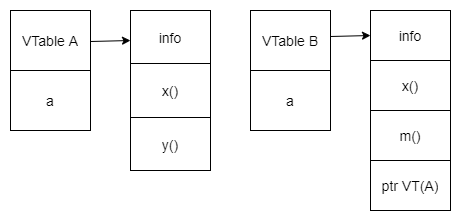
\includegraphics[scale=0.5]{commons/23.png}
			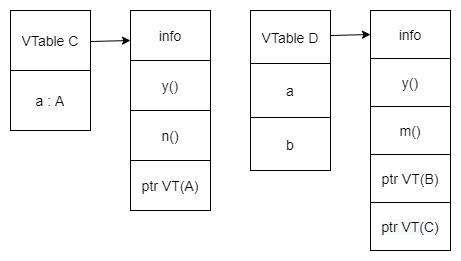
\includegraphics[scale=0.5]{commons/231.png}
		\end{figure}
\end{enumerate}
}
